\section{Requisitos}

% para algum ponto (x, z) precisa sempre gerar o mesmo y função (injetora) (consistência) (ser deterministico)
% (Variedade)
\begin{frame}{Requisitos}
    \begin{itemize}
        \item Determinismo, $ y = f(x, z) $
        \item \alert{Aleatoriedade}
    \end{itemize}
\end{frame}

\begin{frame}{Requisitos}
    \begin{figure}
		\centering
        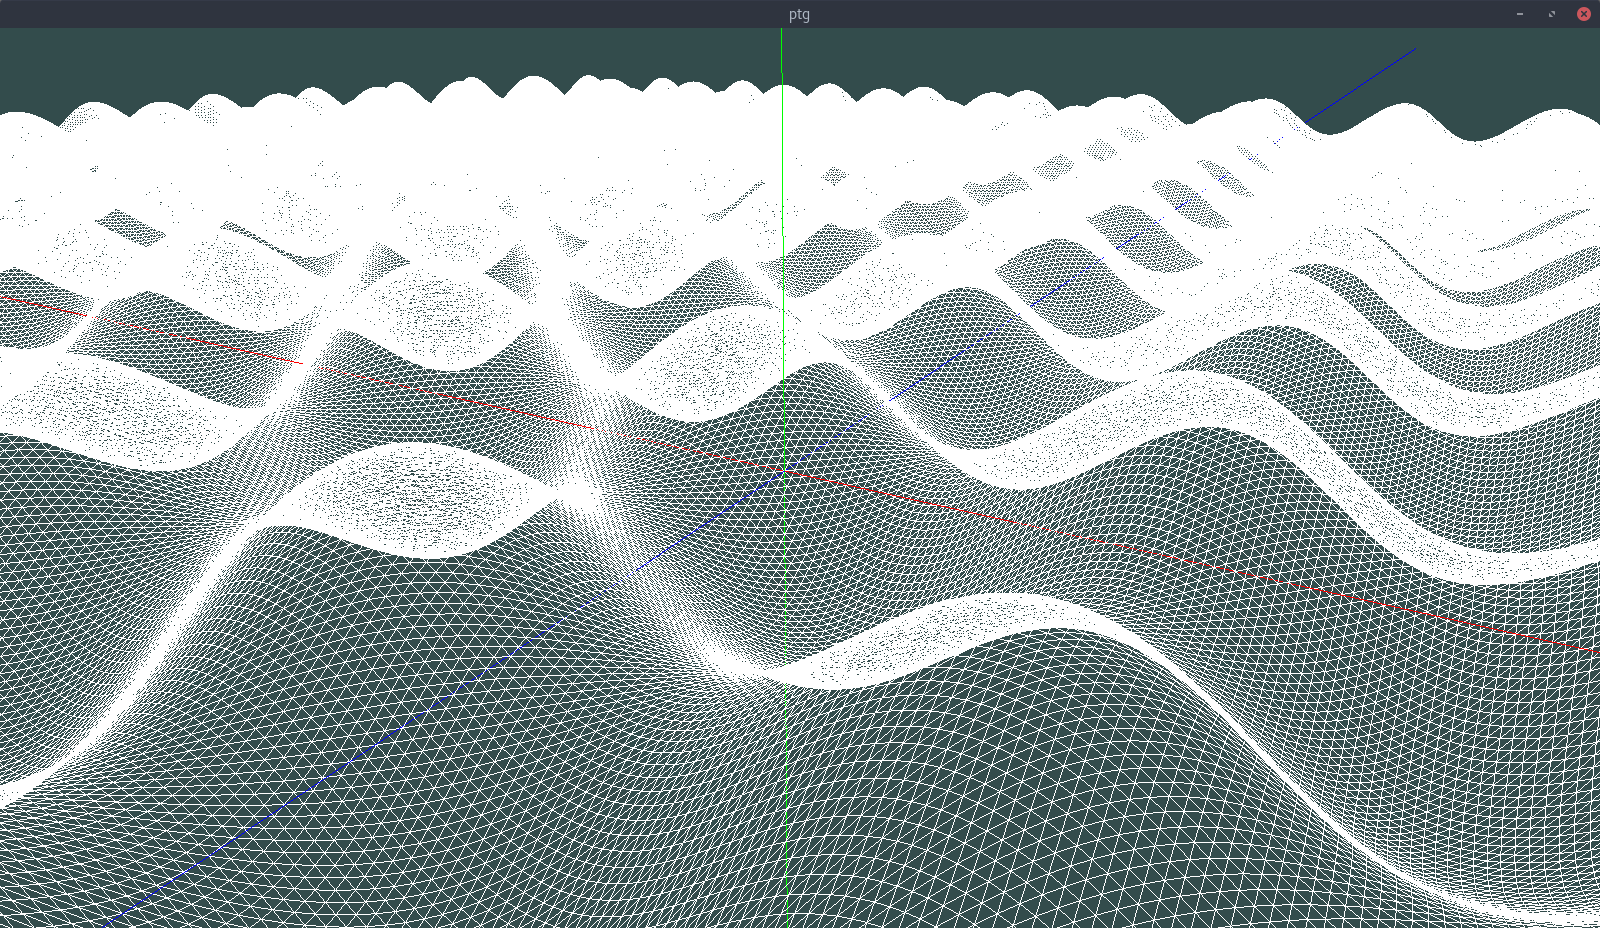
\includegraphics[width=.8\textwidth]{img/intro/sssins.png}
        \caption{$ y = sin(x) + sin(z) $}
    \end{figure}  
\end{frame}
